\subsection{Мера Лебега}

\begin{theorem}
    Классический объем $\lambda_m$ на полукольце ячеек $\mathcal{P}^m$ – 
    $\sigma$-конечная мера.
\end{theorem}

\begin{proof}
    То, что мера $\sigma$-конечная, очевидно – все пространство можно разрезать на счетное количество единичиных ячеек –
    получили счетное объединение ячеек меры 1.

    Надо доказать счетную полуаддитивность $\lambda_m$, т.е. если 
    $(a, b]\subset \bigcup\limits_{n=1}^\infty (a_n, b_n]$, $a, b, a_n, b_n\in \R^m$, то 
    $\lambda_m (a, b]\leq \sum\limits_{n=1}^\infty \lambda_m (a_n, b_n]$

    Зафиксируем $\varepsilon > 0$. Возьмем $[a', b]\subset (a, b]$ и $\lambda_m (a', b']>\lambda_m (a, b]-\varepsilon$.

    Возьмем $(a_n, b_n')\supset (a_n, b_n]$, т.ч. $\lambda_m (a_n, b_n']<\lambda_m (a_n, b_n]+\frac{\varepsilon}{2^n}$.

    Тогда $[a', b]\subset (a, b]\subset \bigcup\limits_{n=1}^\infty (a_n, b_n] \subset \bigcup\limits_{n=1}^\infty (a_n, b_n')
    \Rightarrow[a', b]\subset\bigcup\limits_{n=1}^\infty (a_n, b_n')$ (компакт и открытые множества)

    Выберем конечное подпокрытие: $(a', b]\subset [a', b]\subset\bigcup\limits_{n=1}^N (a_n, b_n')\subset\bigcup\limits_{n=1}^N (a_n, b_n']\Rightarrow$

    $\overset{\text{усил. монот.}}{\Rightarrow} \lambda_m(a, b]- \varepsilon < \lambda_m(a, b]
    \leq \sum\limits_{n=1}^N\lambda_m (a_n, b'_n]< \sum\limits_{n=1}^N(\lambda_m (a_n, b_n] + \frac{\varepsilon}{2^n})<
    \sum\limits_{n=1}^N\lambda_m (a_n, b_n] + \varepsilon\Rightarrow$

    $\Rightarrow\lambda_m(a, b]< \sum\limits_{n=1}^N\lambda_m (a_n, b_n] + 2\varepsilon$ и устремим $\varepsilon$ к нулю.
\end{proof}

\begin{definition}
    Мера Лебега – стандартное продолжение классического объема с полукольца 
    $\mathcal{P}^m$. 
    
    $\sigma$-алгебра, на которую продолжили, – \textit{лебеговская $\sigma$-алгебра}
    и обозначается $\mathcal{L}^m$.
\end{definition}

\begin{remark}
    Из определения стандартного продолжения: $\lambda_m A = \inf \{\sum\limits_{n=1}^\infty \lambda_m P_n \mid P_n\in \mathcal{P}^m\text{ и } A\subset \bigcup\limits_{n=1}^\infty P_n \}$.

    Можно брать и ячейки из $\mathcal{P}^m_{\Q}$, так как каждая ячейка содержится в ячейке сколь угодно близкой меры с рациональными вершинами. (продолжения совпадут).
\end{remark}

\textbf{Свойства меры Лебега:}
\begin{enumerate}
    \item Открытые множества измеримы, мера непустого открытого множества $>0$.
    
    \begin{proof}
        $\mathcal{L}^m\supset \mathcal{B}(\mathcal{P}^m)=\mathcal{B}^m$ содержит все открытые множества.

        Если $G$ – открытое и $\not = \varnothing$, то возьмем $a\in G\Rightarrow
        \exists \underset{\text{ячейка}\subset}{\overline{\text{B}}_r}(a)\subset G$

        $\lambda G\geq \lambda (\text{ячейка})>0$

        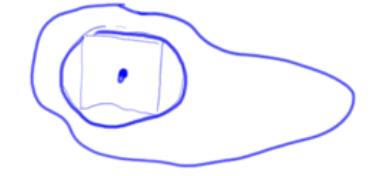
\includegraphics[width=0.15\linewidth]{images/23-09-21-2.png}
    \end{proof}
    \item Замкнутые множества измеримы, мера одноточечного множества = 0.
    
    \begin{proof}
        Накроем точку ячейкой со стороной $\varepsilon$.

        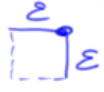
\includegraphics[width=0.05\linewidth]{images/23-09-21-3.png}
        
        $\lambda(\text{точка})\leq \lambda (\text{ячейка}) =\varepsilon^m$
    \end{proof}

    \item Мера ограниченного измеримого множества конечна.
    
    \begin{proof}
        ограниченное множество $\subset$ шар $\subset$ ячейка
    \end{proof}

    \item Всякое измеримое множество – не более чем счетное дизъюнктное объединение множеств конечной меры.
    
    \begin{proof}
        $\R^m =\bigsqcup\limits_{n=1}^\infty P_n$, где $\lambda P_n = 1\Rightarrow E =\bigsqcup\limits_{n=1}^\infty (E\cap P_n)$ и
        $\lambda (E\cap P_n)\leq \lambda P_n = 1$
    \end{proof}

    \item Если $E\subset \R^m$, т.ч. $\forall \varepsilon > 0$ найдутся измеримые множества
    $A_\varepsilon$ и $B_\varepsilon$, т.ч. $A_\varepsilon\subset E \subset B_\varepsilon$ и 
    $\lambda (B_\varepsilon\setminus A_\varepsilon)< \varepsilon$, то $E$ – измеримо.
    
    \begin{proof}
        $A:=\bigcup\limits_{n=1}^\infty A_{\frac{1}{n}}$ и $B:=\bigcap\limits_{n=1}^\infty B_{\frac{1}{n}}\Rightarrow
        A\subset E \subset B$ и $B\setminus A \subset B_{\frac{1}{n}}\setminus A_{\frac{1}{n}}$

        $\lambda (B\setminus A)\leq \lambda (B_{\frac{1}{n}}\setminus A_{\frac{1}{n}})<\frac{1}{n}\Rightarrow \lambda (B\setminus A) = 0$

        $E\setminus A\subset B\setminus A\overset{\text{полнота}}{\Rightarrow} \lambda (E\setminus A)=0$ и $E\setminus A$ измеримо
        $\Rightarrow E= A\cup E\setminus A$ – измеримо
    \end{proof}

    \begin{remark}
        Свойство 5 верно для любой полной меры.
    \end{remark}

    \item Если $E\subset \R^m$, т.ч. $\forall \varepsilon > 0$ найдется измеримое
    $B_\varepsilon\supset E$, т.ч. $\lambda B_\varepsilon< \varepsilon$, то $E$ измеримо и $\lambda E = 0$.

    \begin{proof}
        $A_\varepsilon = \varnothing\overset{\text{п. 5}}{\Rightarrow} E$ – измеримо и $\lambda E\leq \lambda B_\varepsilon < \varepsilon
        \Rightarrow \lambda E = 0$
    \end{proof}

    \item Счетное объединение множеств меры 0 имеет меру 0.
    
    (верно для любой меры, заданной на $\sigma$-алгебре)
    \item Счетное множество имеет меру 0. В частности $\lambda (\Q^m)=0$.
    
    (так как одноточечные множества имеют меру 0)
    \item Множество нулевой меры имеет пустую внутренность.
    
    \begin{proof}
        Если $\Int A\not = \varnothing$, то $A\supset B_r (a)\Rightarrow \lambda A \geq \lambda B_r(a)>0$
    \end{proof}
    \item Если $\lambda e = 0$, то $\forall \varepsilon > 0\ \exists$ такие кубические ячейки $Q_j$, 
    т.ч. $e\subset \bigcup\limits_{j=1}^\infty Q_j$ и $\sum\limits_{j=1}^\infty \lambda Q_j< \varepsilon$.

    \begin{proof}
        $0=\lambda e = \inf \{\sum\limits_{n=1}^\infty \lambda_m P_n \mid e\subset \bigcup\limits_{j=1}^\infty P_j\text{ и }P_j\in \mathcal{P}^m_\Q \}\Rightarrow$

        $\Rightarrow$ можно выбрать $P_j\in \mathcal{P}^m_\Q$, т.ч. $e\subset \bigcup\limits_{j=1}^\infty P_j$ и $\sum \lambda P_j < \varepsilon $

        Рассмотрим ячейку $P_1$, пусть $n=$ НОК знаменателей длин ее сторон. Тогда $P_1$ можно разбить на кубические ячейки со стороной $\frac{1}{n}$.
    \end{proof}

    \item Пусть $m\geq 2$. Гиперплоскость $H_j:= \{x\in \R^m\mid x_j =c\}$ имеет нулевую меру.
    
    \begin{proof}
        $A_n:=(-n, n]^m\cap H_j(c)$, $H_j(c) = \bigcup\limits_{n=1}^\infty A_n$

        Достаточно проверить, что $\lambda A_n =0$: $A_n\subset (-n, n]\times ...\times (-n, n] \times (c - \varepsilon, c]
        \times (-n, n]\times ...\times (-n, n]\Rightarrow \lambda A_n\leq (2n)^{m-1}\cdot \varepsilon$
    \end{proof}

    \item Любое множество, содержащееся в нбчс объединении таких гиперплоскостей, имеет меру 0.
    
    \textit{Комментарий:} счетное объединение множеств нулевой меры имеет нулевую меру.
    
    \item $\lambda (a, b) =\lambda (a, b] = \lambda [a, b]$
    
    \begin{proof}
        $(a, b)\subset (a, b]\subset [a, b]$, $[a, b]\setminus (a, b) \subset$ конечное 
        объединение таких гиперплоскостей.
    \end{proof}

    \begin{remark}~
        \begin{enumerate}
            \item[1.] Существуют несчетные множества нулевой меры.
            
            Если $m\geq 2$, то подойдет $H_j(c)$.

            Если $m= 1$, то подойдет \textit{канторово множество} $\mathbf{K}$.

            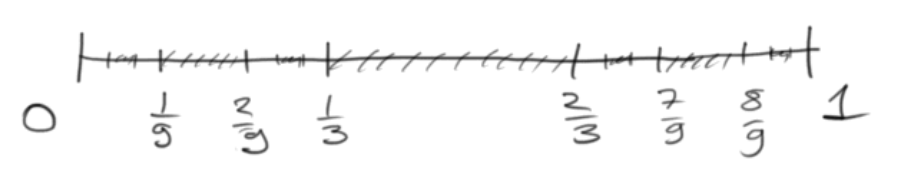
\includegraphics[width=0.35\linewidth]{images/23-09-21-4.png} – то, что осталось, называется канторово множество.

            $\lambda \mathbf{K}+\sum \lambda($выкинутые полуинтервалы$)=\lambda [0, 1)=1$

            $\frac{1}{3}+2\cdot\frac{1}{9}+4\cdot\frac{1}{27}+...+2^{n-1}\cdot\frac{1}{3^n}+...=
            \sum\limits_{n=0}^\infty \frac{2^n}{3^{n+1}}=\frac{1}{3}\sum\limits_{n=0}^\infty (\frac{2}{3})^n=
            \frac{1}{3}\cdot\frac{1}{1-\frac{2}{3}}=1\Rightarrow$ оставшееся множество имеет нулевую меру.

            \textit{Другая интерпретация этого примера:}

            Троичная запись чисел из $[0, 1)$. 
            
            Средний отрезок – первая цифра после запятой 1.

            Два средних отрезка – вторая цифра после запятой 1.

            Продолжая так делать, получим, что останутся в точности те числа, у которых в троичной записи 0 и 2.

            Полученное множество несчетно (так как есть биекция между полученными числами и числами в двоичной записи, 
            просто заменяем 2 на 1).

            \item[2.] Существуют неизмеримые множества. Более того, любое множество положительной
            меры содержит неизмеримое подмножество.

            (пример неизмеримого множества будет позже)
        \end{enumerate}
    \end{remark}
\end{enumerate}

\begin{theorem}
    \textbf{Регулярность меры Лебега.}

    Если $E\subset \R^m$ измеримое множество, то найдется $G$ – открытое, т.ч. $G\supset E$ и $\lambda (G\setminus E) < \varepsilon$.
\end{theorem}

\begin{proof}~
    \begin{enumerate}
        \item $\lambda E < +\infty$, $\lambda E =\inf \{ \sum\limits_{n=1}^\infty \lambda P_n \mid E\subset \cup P_n\text{ и } P_n\in \mathcal{P}^m\}$
        
        Выберем такое покрытие ячейками, что $\sum\limits_{n=1}^\infty \lambda P_n<\lambda E + \varepsilon$.

        $P_n= (a_n, b_n]\subset (a_n, b_n')$, т.ч. $\lambda (a_n, b_n')< \lambda P_n + \frac{\varepsilon}{2^n}$

        $G=\bigcup\limits_{n=1}^\infty (a_n, b_n')\supset \bigcup\limits_{n=1}^\infty P_n \supset E$

        $\lambda (G\setminus E) = \lambda G - \lambda E \leq \sum\limits_{n=1}^\infty \lambda (a_n, b_n') - \lambda E
        \leq \sum\limits_{n=1}^\infty (\lambda P_n + \frac{\varepsilon}{2^n}) - \lambda E = \varepsilon + \sum \lambda P_n - \lambda E < 2\varepsilon$

        \item $\lambda E = +\infty$. Разобьем $E$ в объединение $E_n$, т.ч. $\lambda E_n <+\infty$.

        Возьмем $G_n$ – открытое, т.ч. $E_n\subset G_n$ и $\lambda (G_n \setminus E_n) < \frac{\varepsilon}{2^n}$

        $G:= \bigcup\limits_{n=1}^\infty G_n \supset E$

        $G\setminus E \subset \bigcup\limits_{n=1}^\infty G_n \setminus E_n\overset{\text{полуад.}}{\Rightarrow} \lambda (G\setminus E)\leq \sum\limits_{n=1}^\infty\lambda (G_n \setminus E_n)< 
        \sum\limits_{n=1}^\infty \frac{\varepsilon}{2^n}=\varepsilon$
    \end{enumerate}
\end{proof}

\begin{corollary}~
    \begin{enumerate}
        \item Если $E\subset \R^m$ измеримо, то найдется $F$ – замкнутое, т.ч. 
        $F\subset E$ и $\lambda (E\setminus F)< \varepsilon$.

        \begin{proof}
            Рассмотрим $G\supset X\setminus E$, $\lambda \underbrace{(G\setminus (X\setminus E))}_{=E\setminus (X\setminus G)}< \varepsilon$

            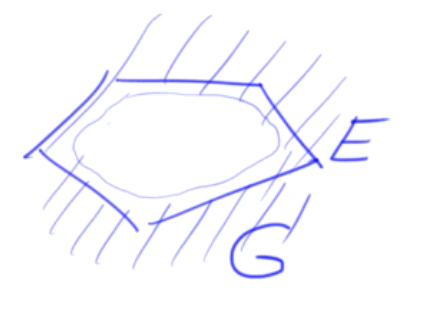
\includegraphics[width=0.2\linewidth]{images/23-09-21-5.png}

            $F:= X\setminus G$ – замкнутое
        \end{proof}

        \item $E$ – измеримое, тогда 
        
        $\lambda E =\inf \{\lambda G\mid G\text{ – открытое и } G\supset E\}$

        $\lambda E = \sup \{\lambda F\mid F\text{ – замкнутое и } F\supset E\}$

        $\lambda E = \sup \{\lambda K\mid K\text{ – компакт и } K\supset E\}$

        \begin{proof}
            $\lambda \underset{\text{замк.}}{F}=\lim\limits_{n\rightarrow \infty} \lambda (\underset{\text{компакты}}{[-n, n]^m} \cap F)$ – непрер. меры снизу
        \end{proof}
        
        \item Если $E$ – измеримо, то существует $K_n$ – компакты, т.ч. $K_1 \subset K_2 \subset ...$ и $e$ – нулевой
        меры, т.ч. $E=\bigcup\limits_{n=1}^\infty K_n\cup e$.

        \begin{proof}
            Берем компакты $\tilde{K_n}$, т.ч. $\lambda\tilde{K_n} \rightarrow \lambda E$.

            Если $\lambda E<+\infty $, то $\lambda (E\setminus \tilde{K_n})\rightarrow 0\Rightarrow \lambda (E\setminus \bigcup\limits_{n=1}^\infty \tilde{K_n}) = 0
            \Rightarrow e:=\bigcup\limits_{n=1}^\infty \tilde{K_n}$ и $K_n=\tilde{K_1}\cup \tilde{K_2}\cup ... \cup \tilde{K_n}$ подходят.

            Если $\lambda E\rightarrow +\infty $, то $E=\sqcup E_n$, т.ч. $\lambda E_n < +\infty$.

            $E_n=\bigcup\limits_{j=1}^\infty K_n\cup e_n$, $\lambda e_n = 0$, $K_{nj}$ – компакты.
        \end{proof}
    \end{enumerate}
\end{corollary}

\begin{theorem}
    При сдвиге измеримого множества его измеримость и мера сохраняются. 
\end{theorem}

\begin{proof}
    Сдвиг на вектор $v$: $\mu E:=\lambda (v + E)$ на ячейках 
    $\lambda$ и $\mu$ совпадают $\Rightarrow$ по единственности продолжения они совпадают.
\end{proof}

\begin{theorem}
    Пусть $\mu$ мера на $\mathcal{L}^m$, т.ч.

    \begin{enumerate}
        \item Инвариантна относительно сдвигов.
        \item Мера $\mu$ для каждой ячейки конечна = мера любого ограниченного измеримого множеcтва конечна.
    \end{enumerate}

    Тогда найдется $k\in [0, +\infty)$, т.ч. $\mu = k\cdot \lambda$ (т.е. $\mu E = k\lambda E$).
\end{theorem}

\begin{proof}
    Положим $Q:= (0, 1]^m$. Тогда $k := \mu Q$.

    \begin{enumerate}
        \item Случай $k=1$
        
        Надо доказать, что $\mu =\nu$. Для этого достаточно совпадения на $\mathcal{P}^m_\Q$.
        Любая такая ячейка складывается из кубиков со стороной вида $\frac{1}{n}$, т.е. достаточно 
        совпадения на кубике $Q_n =(0, \frac{1}{n}]^m$.

        $\lambda (0, \frac{1}{n}]^m= (\frac{1}{n})^m$

        $\mu (0, \frac{1}{n}]^m\overset{?}{=} (\frac{1}{n})^m$

        Ячейка $Q$ есть объединение $n^m$ попарно не пересекающихся сдвигов ячейки $Q_n$:

        $\mu (0, \frac{1}{n}]^m= \frac{\mu Q}{n^m}=(\frac{1}{n})^m$

        \item Случай $k\not = 0$
        
        $\tilde{\mu}:=\frac{1}{k}\mu$. Тогда $\tilde{\mu} Q=1$, $\tilde{\mu}$ инваривантна
        относительно сдвигов $\Rightarrow\tilde{\mu}=\lambda$

        \item Случай $k = 0$
        
        $\R^m$ – счетное объединение сдвигов $Q\Rightarrow\mu (\R^m)=0$
    \end{enumerate}
\end{proof}

\begin{theorem}
    Мера Лебега инвариантна относительно движения.
\end{theorem}

\begin{proof}
    Надо доказать, что мера Лебега не меняется при вращении.

    Пусть $U$ – поворот. Рассмотрим $\mu E := \lambda (UE)$ – мера на $\mathcal{L}^m$ и докажем, что $\nu=\mu$.

    $\mu$ конечна на ограниченных множествах и инвариантна относительно сдвигов.
    $\mu(E + v) = \lambda (U(E+v))=\lambda (UE+Uv)=\lambda (UE)=\mu E$
    
    Тогда по теореме $\mu=k\lambda$ для $k\in [0, +\infty)$. А так как единичный шар переходит в
    себя при вращении, то $ k=1$.
\end{proof}

\subsubsection*{Пример неизмеримого множества}

Пусть $x, y\in (0, 1]$. Определим класс эквивалентности $x\tilde y$, если $x-y\in \Q$

$A$ – множество, в которое взяли по одному представителю из каждого класса эквивалентности. 

Построенное множество $A$ неизмеримо.

\begin{proof}
    От противого. Пусть $A$ измеримо.

    \begin{enumerate}
        \item $\lambda A = 0$. Тогда $(0, 1]\subset \bigcup\limits_{x\in \Q} 
        \overset{\text{мн-ва нулевой меры}}{(A+x)}\Rightarrow \lambda (0, 1]=0$, противоречие.

        \item $\lambda A > 0$. Тогда $\bigsqcup\limits_{x\in \Q} (A+x)\subset (0, 2]\Rightarrow 2 
        \geq \sum\limits_{x\in \Q, 0\leq x \leq 1} \overset{\text{все меры одинак.}}{\lambda(A+x)}$, противоречие.
    \end{enumerate}
\end{proof}

\begin{theorem}
    Пусть $G\subset \R^m$ открытое, $\Phi : G\rightarrow \R^m$ непрерывно дифференцируемо. Тогда:
    \begin{enumerate}
        \item Если $e\subset G$, т.ч. $\lambda e=0$, то $\Phi(e)$ измеримо и $\lambda (\Phi(e)) =0$.
        \item Если $E\subset G$, т.ч. $E$ – измеримо, то $\Phi(E)$ измеримо.
    \end{enumerate}
\end{theorem}

\begin{proof}~
    \begin{enumerate}
        \item \textbf{Шаг 1.} Пусть $e\subset P\subset \Cl P\subset G$, где $P$ – ячейка.
        
        $\|\Phi'(x)\|$ – непрерывна на компакте $\Cl P\Rightarrow \|\Phi'(x)\|$ ограничена
        на $\Cl P$. 
        
        Пусть $\|\Phi'(x)\|\leq M$. Тогда $\|\Phi'(x)-\Phi'(y)\|\leq M\|x-y\|$ $\forall x, y\in \Cl P$.

        Накроем $e$ кубическими ячейками $Q_j$ так, что $\sum \lambda Q_j<\varepsilon$.

        Пусть $h_j$ – ребро $Q_j$. Тогда если $x, y\in Q_j$, то $\|x - y\|\leq \sqrt{m}h_j\Rightarrow
        \|\Phi'(x)-\Phi'(y)\|\leq M\sqrt{m}h_j\Rightarrow \Phi(Q_j)$ содержится в шаре радиуса $M\sqrt{m}h_j\Rightarrow
        \Phi(Q_j)$ содержится в кубе со стороной $2M\sqrt{m}h_j$

        $\Phi(e)\subset \bigcup\Phi(Q_j)$, $\sum \lambda (\Phi(Q_j))\leq \sum (2M\sqrt{m}h_j)^m=(2M\sqrt{m})^m 
        \sum \underset{=\lambda Q_j}{h_j^m}=(2M\sqrt{m})^m \sum \lambda Q_j<(2M\sqrt{m})^m\cdot \varepsilon$

        \textbf{Шаг 2.} $e$ произвольное, $G=\bigsqcup P_k$, где $P_k$ – ячейки, т.ч. $\Cl P_k\subset G$

        $e_k:=e\cap P_k\Rightarrow$ по шагу 1 $\lambda e_k=0\Rightarrow \lambda e=0$

        \item $E=e\cup \bigcup K_n$, где $\lambda e=0$ и $K_n$ – компакт $\Rightarrow\Phi(E)=
        \underset{\text{нулев. мера}}{\Phi(e)}\cup \underset{\text{компакты}}{\Phi(K_n)}$ все множества измеримы
    \end{enumerate}
\end{proof}


\begin{theorem}
    \textbf{Теорема об изменении меры лебега при линейном отображении.}

    Пусть $T:\R^m\rightarrow \R^m$ линейное, $E$ – измеримое. Тогда $\lambda(T(E))=|\det T|\cdot \lambda E$.
\end{theorem}

\begin{proof}
    $\mu E := \lambda (T(E))$ инвариантнa относительно сдвигов и конечна на ограниченных множествах 
    $\Rightarrow \mu = k\lambda$ для $k=\lambda (T((0, 1]^m))$. Это $|\det T|$ (из алгебры).
\end{proof}


\subsection{Измеримые функции}

\begin{definition}
    Пусть $f: E\rightarrow \overline{\R}$, $a\in \R$.

    $E\{f<a\}:= \{x\in E\mid f(x) < a\}=f^{-1}((-\infty, a))$

    $E\{f\leq a\}:= \{x\in E\mid f(x) \leq a\}=f^{-1}((-\infty, a])$

    $E\{f\leq a\}$ и $E\{f\leq a\}$ 

    Все это – \textit{лебеговые множества функции $f$}.
\end{definition}

\begin{theorem}
    Пусть $E$ – измеримое, $f:E\rightarrow \overline{\R}$. Следующие условия 
    равносильны:

    \begin{enumerate}
        \item $E\{f<a\}$ измеримо $\forall a\in \R$.
        
        \item $E\{f\leq a\}$ измеримо $\forall a\in \R$.
        
        \item $E\{f>a\}$ измеримо $\forall a\in \R$.
        
        \item $E\{f\geq a\}$ измеримо $\forall a\in \R$.
    \end{enumerate}
\end{theorem}

\begin{proof}~

    \begin{itemize}
        \item $E\{f<a\} = E\setminus E\{f\geq a\}\Rightarrow 1\Leftrightarrow 4$
        
        \item $E\{f>a\} = E\setminus E\{f\leq a\}\Rightarrow 2\Leftrightarrow 3$
        
        \item $2\Rightarrow 1$: $E\{f<a\} =\bigcup\limits_{n=1}^\infty E\{f\leq a-\frac{1}{n}\}$
        
        \item $4\Rightarrow 3$: $E\{f>a\} =\bigcup\limits_{n=1}^\infty E\{f\geq a+\frac{1}{n}\}$
    \end{itemize}
\end{proof}

\begin{definition}
    $f:E\rightarrow \overline{\R}$ – \textit{измерима}, если все ее лебеговы множества 
    при всех $a\in \R$ измеримы.
\end{definition}

\begin{example}~
    \begin{enumerate}
        \item Константа (на измеримом множестве)
        
        \item $E\supset A$ – измеримы
        
        $\mathbf{1}_A(x):= \left\{\begin{array}{ll}
            1, & \text{если } x\in A \\
            0, & \text{если } x\in E \setminus A \\ 
        \end{array}\right.$, $\mathbf{1}_A :E \rightarrow \R$ – \textit{характеристическая функция}.

        \item $E\in \mathcal{L}^m$, $f:E\rightarrow \R$ непрерывна $\Rightarrow f$ – 
        измерима относительно $\mathcal{L}^m$.

        \begin{proof}
            Достаточно измеримости множеств $E\{f<a\}=f^{-1}(\underset{\text{открытое}}{(-\infty, a)})$ – открытые 
            множества $\Rightarrow$ они из  $\mathcal{L}^m$.
        \end{proof}
    \end{enumerate}
\end{example}

\subsection*{Свойства измеримых функций:}

\begin{enumerate}
    \item Если $f:E\rightarrow \overline{\R}$ измерима, то $E$ – измеримое множество.
    
    \begin{proof}
        $E=\underset{=E\{f<+\infty\}}{\bigcup\limits_{n=1}^\infty E\{f < n\}}\cup \underset{=E\{f=+\infty\}}{\bigcap\limits_{n=1}^\infty E\{f > n\}}$
    \end{proof}

    \item Если $f:E\rightarrow \overline{\R}$ измерима, $\underset{\text{измеримо}}{E_0}\subset E\Rightarrow f\mid_{E_0}$
    – измеримо.

    \begin{proof}
        $E_0\{f\mid_{E_0}< a\}=E_0\cap E\{f < a\}$
    \end{proof}
\end{enumerate}